% !TeX root = booklet-01.tex
\section{اجرای چندچرخه‌ای و مسیر داده}
\label{sec:mips-micro}
\subsection{چرا \lr{Multicycle}؟}
در پیاده‌سازی \lr{Multicycle}، یک دستور در چند چرخه اجرا می‌شود و یک منبع
می‌تواند در چرخه‌های مختلف چند کار انجام دهد. در این مثال، همان \lr{ALU}
ابتدا \lr{PC} را افزایش می‌دهد، سپس آدرس یا نتیجه حسابی را محاسبه می‌کند.
ثبات‌های میانی، نتیجه را تا زمان مصرف نگه می‌دارند
\cite[بخش \secnum{۱.۷.۲}]{weste}.
صرف چندچرخه‌ای بودن، اجرای هم‌زمان چند دستور یا \lr{Pipeline} را ثابت نمی‌کند؛
این کنترل‌کننده یک دستور را به‌ترتیب مراحلش جلو می‌برد.

\lr{Datapath} شامل مسیرهای داده، \lr{MUX}ها، ثبات‌ها، \lr{Register File}
و \lr{ALU} است. \lr{Controller} با دیدن نوع دستور، حالت جاری و پرچم‌هایی
مثل \code{Zero}، انتخاب مسیر و اجازه نوشتن را مشخص می‌کند.
شکل \ref{fig:mips-overview} جداسازی این دو مسئولیت را نشان می‌دهد.

\begin{figure}[ht]
\centering
\begin{latin}
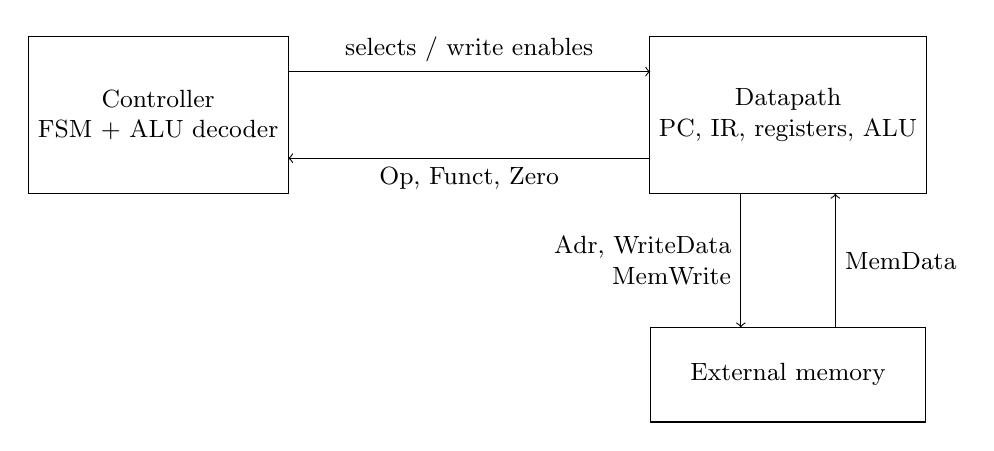
\begin{tikzpicture}[font=\small]
\node[draw,minimum width=3.3cm,minimum height=2cm,align=center] (c) at (0,0) {Controller\\FSM + ALU decoder};
\node[draw,minimum width=3.5cm,minimum height=2cm,align=center] (d) at (8,0) {Datapath\\PC, IR, registers, ALU};
\draw[->] (1.65,0.55)--node[above] {selects / write enables}(6.25,0.55);
\draw[->] (6.25,-0.55)--node[below] {Op, Funct, Zero}(1.65,-0.55);
\node[draw,minimum width=3.5cm,minimum height=1.2cm] (m) at (8,-3.3) {External memory};
\draw[->] (7.4,-1)--node[left,align=right] {Adr, WriteData\\MemWrite}(7.4,-2.7);
\draw[->] (8.6,-2.7)--node[right] {MemData}(8.6,-1);
\end{tikzpicture}
\end{latin}
\caption{نمای فشرده آموزشی مسیر داده و کنترل، بر پایه شکل‌های \secnum{۱.۵۳}
و \secnum{۱.۵۶} کتاب \cite{weste}. این شکل همه سیم‌ها و \lr{MUX}های شکل اصلی را رسم نمی‌کند؛
انتخاب‌های آن‌ها در جدول \ref{tab:mips-selects} آمده‌اند.}
\label{fig:mips-overview}
\end{figure}

\subsection{نقش ثبات‌های میانی}
\lr{IR} دستور ۳۲بیتی را نگه می‌دارد؛ ثبات \code{Data} بایت خوانده‌شده حافظه
را برای نوشتن بعدی در ثبات مقصد حفظ می‌کند.
ثبات‌های \code{A} و \code{B} دو داده خوانده‌شده از \lr{Register File} را
در اختیار \lr{ALU} می‌گذارند. \code{ALUOut} نیز نتیجه مرحله قبل، مانند
آدرس موثر یا نتیجه حسابی را نگه می‌دارد.
بنابراین \code{ALUResult}، خروجی محاسبه جاری و \code{ALUOut}، مقدار ثبت‌شده‌اند؛
هم‌نام یا هم‌زمان بودن مقدارشان را نباید فرض کرد.

\lr{MUX} ورودی اول \lr{ALU} بین \lr{PC} و \code{A} انتخاب می‌کند؛
ورودی دوم می‌تواند \code{B}، ثابت یک، بخش ثابت دستور یا ثابت ضرب‌شده در چهار باشد.
\code{PCEn} اجازه نوشتن \lr{PC} است و در مدل شکل کتاب از رابطه زیر می‌آید:
\begin{equation}\label{eq:mips-pcen}
\mathrm{PCEn}=\mathrm{PCWrite}+(\mathrm{Branch}\cdot\mathrm{Zero}).
\end{equation}
علامت جمع اینجا \lr{OR} منطقی است. \code{PCWrite} نوشتن بی‌قید به برابری
و \code{Branch} همراه \code{Zero} نوشتن مشروط را فعال می‌کند.
در \code{BEQ}، تفریق دو عملوند اگر صفر شود، برابری را نشان می‌دهد.

\subsection{معنای دقیق انتخاب‌گرها}
جدول \ref{tab:mips-selects} قرارداد شکل \secnum{۱.۵۳} کتاب را باز می‌کند.
اعداد انتخاب، کدهای همان طراحی‌اند و استاندارد همگانی سیگنال‌های هم‌نام نیستند.
\begin{table}[ht]
\centering
\caption{انتخاب مسیرها در \lr{Datapath} آموزشی کتاب}
\label{tab:mips-selects}
\begin{tabularx}{\textwidth}{lX}
\toprule
کنترل & انتخاب در شکل کتاب\\
\midrule
\code{IorD}&\code{0}: آدرس حافظه از \lr{PC}؛ \code{1}: از \code{ALUOut}\\
\code{ALUSrcA}&\code{0}: \lr{PC}؛ \code{1}: ثبات موقت \code{A}\\
\code{ALUSrcB}&\code{00}: \code{B}؛ \code{01}: یک؛ \code{10}: ثابت داده؛ \code{11}: ثابت ضرب‌شده در چهار\\
\code{PCSrc}&\code{00}: \code{ALUResult}؛ \code{01}: \code{ALUOut}؛ \code{10}: مقصد پرش\\
\code{RegDst}&\code{0}: فیلد \code{rt}؛ \code{1}: فیلد \code{rd}\\
\code{MemtoReg}&\code{0}: \code{ALUOut}؛ \code{1}: ثبات \code{Data}\\
\code{IRWrite[3:0]}&چهار اجازه نوشتن مستقل برای چهار بایت \lr{IR}\\
\code{RegWrite}&اجازه نوشتن در \lr{Register File}\\
\code{MemWrite}&اجازه نوشتن حافظه بیرونی\\
\bottomrule
\end{tabularx}
\end{table}
در آدرس‌های هشت‌بیتی، خروجی محاسبات آدرس به هشت بیت محدود است.
برای داده، ثابت از بیت‌های پایین دستور وارد مسیر هشت‌بیتی می‌شود؛
برای شاخه، مسیر شیفت چپ دو بیت جداگانه در شکل مشخص است.
وجود نام \code{MemtoReg} به معنی انتخاب همیشگی حافظه نیست؛ مقدار کنترل مسیر را تعیین می‌کند.

\subsection{چهار \lr{Fetch} و ترتیب بایت‌های \lr{IR}}
حالت‌های صفر تا سه کنترل‌کننده، هرکدام یک بایت را از آدرس \lr{PC} می‌خوانند
و در یک بخش \lr{IR} می‌نویسند. در همان چرخه، \lr{ALU} با انتخاب
\code{ALUSrcA=0} و \code{ALUSrcB=01}، مقدار \(PC+1\) را تولید می‌کند.
\code{PCWrite=1} و \code{PCSrc=00} اجازه ثبت آن را می‌دهند
\cite[مثال \secnum{۱.۵}]{weste}.

در حالت اول، \code{IRWrite0} بایت کم‌ارزش را ثبت می‌کند؛ سه حالت بعدی
به‌ترتیب بایت‌های دیگر را می‌نویسند. برای کد \code{20030008} در حافظه بایتی،
ترتیب \code{08, 00, 03, 20} در آدرس‌های پیاپی با این قرارداد سازگار است.
پس کد نمایش‌داده‌شده ۳۲بیتی با ترتیب نمایش بایت‌های حافظه یکی نیست.
بعد از چهار انتقال، دستور کامل و \lr{PC} آماده نشانی دستور بعدی است.

متن مثال کتاب نام \code{MemRead} را نیز هنگام توصیف خواندن می‌آورد؛
ولی رابط نهایی جدول \secnum{۱.۹} پایه مستقلی با این نام ندارد.
در این جزوه خواندن را در چارچوب حافظه ساده همان شکل تفسیر می‌کنیم و
پایه جدیدی به رابط اضافه نمی‌کنیم. برای حافظه واقعی با پروتکل یا زمان انتظار،
قرارداد خواندن باید جداگانه مشخص شود.

\section{ماشین حالت و اجرای دستورها}
\subsection{مفهوم \lr{FSM} و جدول حالت‌های کتاب}
\lr{Finite State Machine (FSM)} مجموعه محدودی از حالت‌ها، قانون انتقال
و خروجی‌های کنترلی دارد. حالت، مرحله اجرای فعلی را نگه می‌دارد؛
\code{op} مشخص می‌کند پس از \lr{Decode} به کدام مسیر برویم.
جدول \ref{tab:mips-fsm} حالت‌های شکل \secnum{۱.۵۴} را خلاصه می‌کند
\cite{weste}.

\begin{table}[ht]
\centering
\caption{حالت‌های رسم‌شده کنترل‌کننده کتاب؛ شماره‌ها شناسه حالت‌اند، نه شماره چرخه همه دستورها.}
\label{tab:mips-fsm}
\begin{tabularx}{\textwidth}{cXX}
\toprule
حالت & عمل اصلی & مسیر بعدی\\
\midrule
۰، ۱، ۲، ۳&\lr{Fetch} چهار بایت و افزایش بایتی \lr{PC}&به‌ترتیب تا حالت ۴\\
۴&\lr{Decode}، خواندن دو ثبات و محاسبه مقصد احتمالی شاخه&با توجه به \code{op} به ۵، ۹، ۱۱ یا ۱۲\\
۵&محاسبه آدرس موثر برای \code{LB/SB}&برای \code{LB} به ۶؛ برای \code{SB} به ۸\\
۶&خواندن بایت حافظه و ثبت در \code{Data}&۷\\
۷&نوشتن داده حافظه در ثبات مقصد&۰\\
۸&نوشتن بایت \code{B} در حافظه&۰\\
۹&اجرای عمل \lr{R-type} و ثبت نتیجه&۱۰\\
۱۰&نوشتن \code{ALUOut} در ثبات مقصد&۰\\
۱۱&مقایسه برای \code{BEQ} و تغییر مشروط \lr{PC}&۰\\
۱۲&ثبت مقصد \code{J} در \lr{PC}&۰\\
\bottomrule
\end{tabularx}
\end{table}

حالت‌های اجرای \code{ADDI} در شکل کتاب رسم نشده‌اند و به‌عنوان تمرین
خواننده باقی گذاشته شده‌اند. بنابراین جدول را کنترل‌کننده کامل همه ده دستور
اعلام نمی‌کنیم. مسیر \code{ADDI} برای اجرای برنامه لازم است؛ از نظر رفتاری
باید \code{A} را با ثابت جمع و نتیجه را در \code{rt} ثبت کند، اما این توصیف
جای پیاده‌سازی و تایید حالت‌های اضافه را نمی‌گیرد.

\subsection{ردگیری کامل \code{SUB}}
برای \code{sub \$5, \$4, \$5}، چهار \lr{Fetch} ابتدا \lr{IR} را کامل می‌کنند.
در حالت ۴، فیلدهای \code{rs} و \code{rt} ثبات‌های چهار و پنج را می‌خوانند
و در \code{A} و \code{B} قرار می‌دهند.
محاسبه جانبی مقصد شاخه در همین حالت برای این دستور مصرف نمی‌شود.

در حالت ۹، \code{ALUSrcA=1} و \code{ALUSrcB=00} دو داده را به
\lr{ALU} می‌فرستند. \code{ALUOp=10} یعنی نوع عمل از \code{funct}
تعیین شود؛ برای \code{funct=100010}، کنترل \code{110} تفریق را انتخاب می‌کند.
نتیجه در \code{ALUOut} ثبت می‌شود.
در حالت ۱۰، \code{RegDst=1} مقصد \code{rd}،
\code{MemtoReg=0} داده \code{ALUOut} و \code{RegWrite=1} اجازه نوشتن را
انتخاب می‌کنند؛ سپس کنترل به \lr{Fetch} بعدی برمی‌گردد
\cite[مثال \secnum{۱.۵}، صفحات چاپی ۳۷ و ۳۸]{weste}.

پس این \lr{R-type} در مدل بدون انتظار حافظه، چهار \lr{Fetch}، یک \lr{Decode}،
یک \lr{Execute} و یک \lr{Write-back}، یعنی هفت چرخه دارد.
عبارت «سه مرحله برای جمع یا تفریق» پس از \lr{Fetch}، نباید با سه چرخه برای کل دستور اشتباه شود.

\subsection{چرا شاخه به نتیجه ثبت‌شده قبلی نیاز دارد؟}
در حالت ۴، \lr{ALU} از \lr{PC} بعد از \lr{Fetch} و ثابت ضرب‌شده در چهار،
مقصد احتمالی را می‌سازد و در \code{ALUOut} قرار می‌دهد.
در حالت ۱۱، همان \lr{ALU} برای تفریق \code{A-B} استفاده می‌شود تا
\code{Zero} به دست آید؛ مقصد از \code{ALUOut} قبلی انتخاب می‌شود، نه خروجی
تفریق جاری. این استفاده دوباره از منبع، دلیل اهمیت ثبات موقت است.

اگر داده‌ها برابر باشند، \code{Branch=1} و \code{Zero=1} طبق رابطه
\eqref{eq:mips-pcen}، \lr{PC} را با مقصد شاخه به‌روزرسانی می‌کنند؛
اگر برابر نباشند، \lr{PC} همان آدرس بعد از \lr{Fetch} را نگه می‌دارد.
در نمونه هشت‌بیتی، تفریق صفر دقیقاً برابری دو الگوی هشت‌بیتی را نشان می‌دهد.

\subsection{تفاوت مسیر \code{LB} و \code{SB}}
هر دو پس از \lr{Decode} در حالت ۵، آدرس \(R_a+\mathrm{imm}\) را
در \code{ALUOut} ثبت می‌کنند. با \code{IorD=1}، آدرس حافظه از این ثبات می‌آید.
\code{LB} در حالت ۶ بایت را می‌خواند و در حالت ۷ با
\code{RegDst=0, MemtoReg=1, RegWrite=1} در \code{rt} می‌نویسد.
\code{SB} در حالت ۸ داده \code{B} را با \code{MemWrite=1} به حافظه می‌دهد.
بنابراین \code{LB} هشت و \code{SB} هفت چرخه در نمودار رسم‌شده نیاز دارند.
\code{BEQ} و \code{J} هرکدام با چهار \lr{Fetch}، \lr{Decode} و یک مرحله نهایی، شش چرخه دارند.

\subsection{\lr{Decode} عمل \lr{ALU} را با حالت اجرا یکی نگیریم}
جدول \ref{tab:mips-aludec} از جدول \secnum{۱.۸} کتاب گرفته شده است.
\code{x} یعنی مقدار آن فیلد برای همان تصمیم استفاده نمی‌شود؛ به معنی
ایجاد حالت ناشناخته در همه خروجی‌ها نیست.
\begin{table}[ht]
\centering
\caption{تفکیک \code{ALUOp} تولیدشده توسط \lr{FSM} از \code{ALUControl} محلی}
\label{tab:mips-aludec}
\begin{tabular}{llll}
\toprule
\code{ALUOp}&\code{funct}&\code{ALUControl}&عمل\\
\midrule
\code{00}&\code{x}&\code{010}&\code{ADD}\\
\code{01}&\code{x}&\code{110}&\code{SUB}\\
\code{10}&\code{100000}&\code{010}&\code{ADD}\\
\code{10}&\code{100010}&\code{110}&\code{SUB}\\
\code{10}&\code{100100}&\code{000}&\code{AND}\\
\code{10}&\code{100101}&\code{001}&\code{OR}\\
\code{10}&\code{101010}&\code{111}&\code{SLT}\\
\code{11}&\code{x}&\code{x}&تعریف‌نشده در جدول\\
\bottomrule
\end{tabular}
\end{table}
خود \lr{FSM} حالت‌دار است، ولی \lr{ALU Decoder} می‌تواند یک مدار
\lr{Combinational} از کد عمل و \code{funct} باشد.
یکسان بودن \lr{ALUControl} برای جمعِ \lr{Fetch} و جمعِ دستور،
به معنی یکسان بودن بقیه انتخاب‌ها و مقصد ثبت نیست.
